\documentclass{article}
\usepackage{amsmath}
\usepackage{float}
%\usepackage{babel}
\usepackage{graphicx}
\usepackage{amssymb}
\usepackage{enumerate}
\usepackage[top=1in, bottom=1.5in, left=1.5in, right=1.5in]{geometry}

\begin{document}
\title{\huge Image Compression Through Multi-Scale Learned Dictionaries \\  { \large  \textsc{patch size experiment report-DRAFT}}}
\date{August 3, 2014}

\author{{\Large Oron Anschel}\vspace{0.2cm}   \\ {Supervisor}: Jeremias Sulam \hspace{2cm} Co-Supervisor: Ori Bryt }


\maketitle
\nopagebreak

\section{Summary}
Definitions:
\begin{itemize}
\item BBP  - Byte per pixel 
\item NNZD - Number of non zeros entries in all sparse dictionaries.
\item NNZG - Number of non zeros entries in all GAMMAs.
\end{itemize}

The compression scheme is based on 6 levels of wavelet decomposition, each level has a sparse dictionary and a GAMMA (sparse representation).
In this experiment one for each level we hold all the other parameters and change the size of the patch size, notice that dictionary redundancy is kept those when the patch size grows there are more columns/rows in the dictionary.

Original images are 512x512
level 1 is corresponding to 256x256 coefficients sub-bands images.
level 6 is corresponding to 8x8     coefficients sub-bands images.
\newpage 
\section{PSNR=25 results}
\begin{figure}[h]
\centering
    \begin{center}
       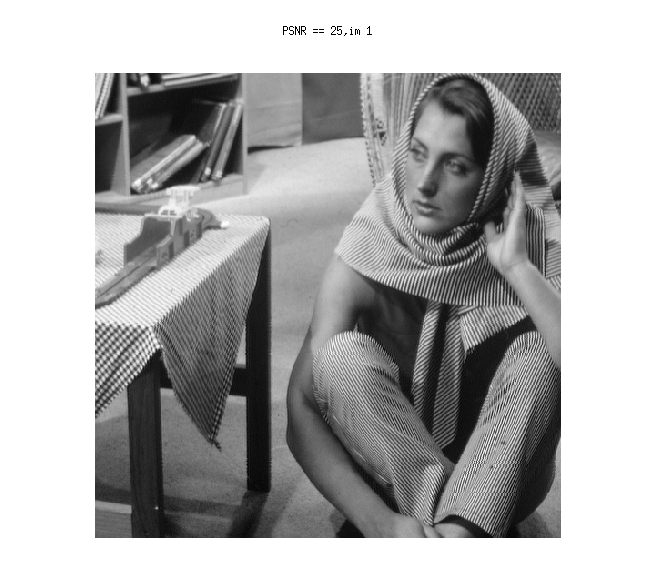
\includegraphics[scale=0.3]{1.png}
    \end{center}
    \noindent
\end{figure}
\begin{figure}[h]
\centering
  
    \begin{center}
       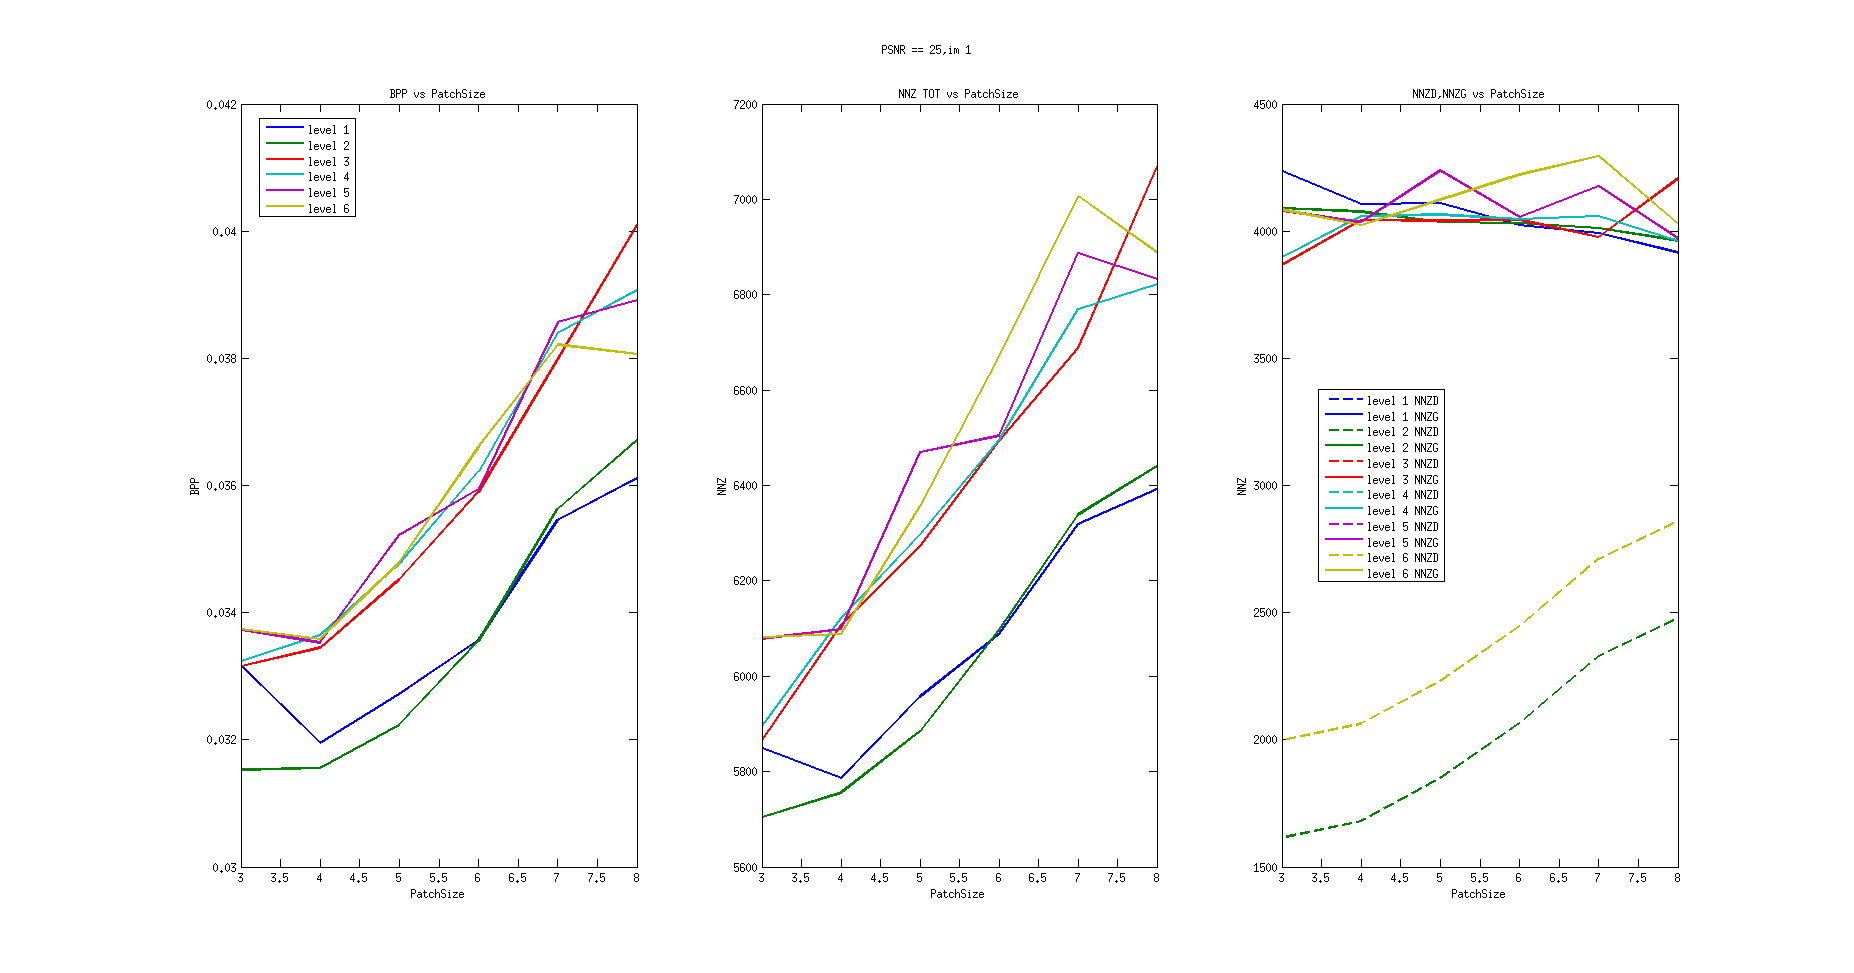
\includegraphics[width=180mm]{fig1L.png}
     
    \end{center}
\end{figure}
3 Images results are presented, other images results are similar.
it can be observed here that, for low PSNR smaller patch size are better, we can see in the right graph that this is due to the fact more atoms are added to the dictionary as the the patch size grows but GAMMA does has less columns, but the number of total coefficients is decreasing only in level 1-2 and not as fast as dictionary atoms are added.

\newpage 
\begin{figure}[h]
\centering
    \begin{center}
       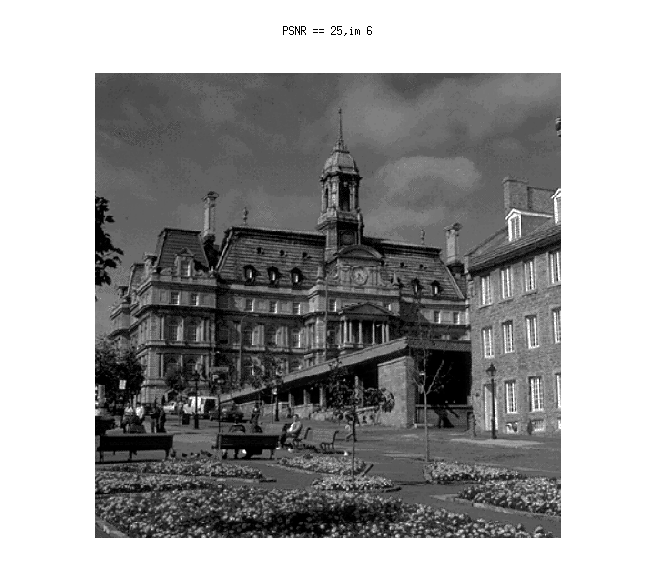
\includegraphics[scale=0.3]{6.png}
    \end{center}
    \noindent
\end{figure}
\begin{figure}[h]
\centering
  
    \begin{center}
       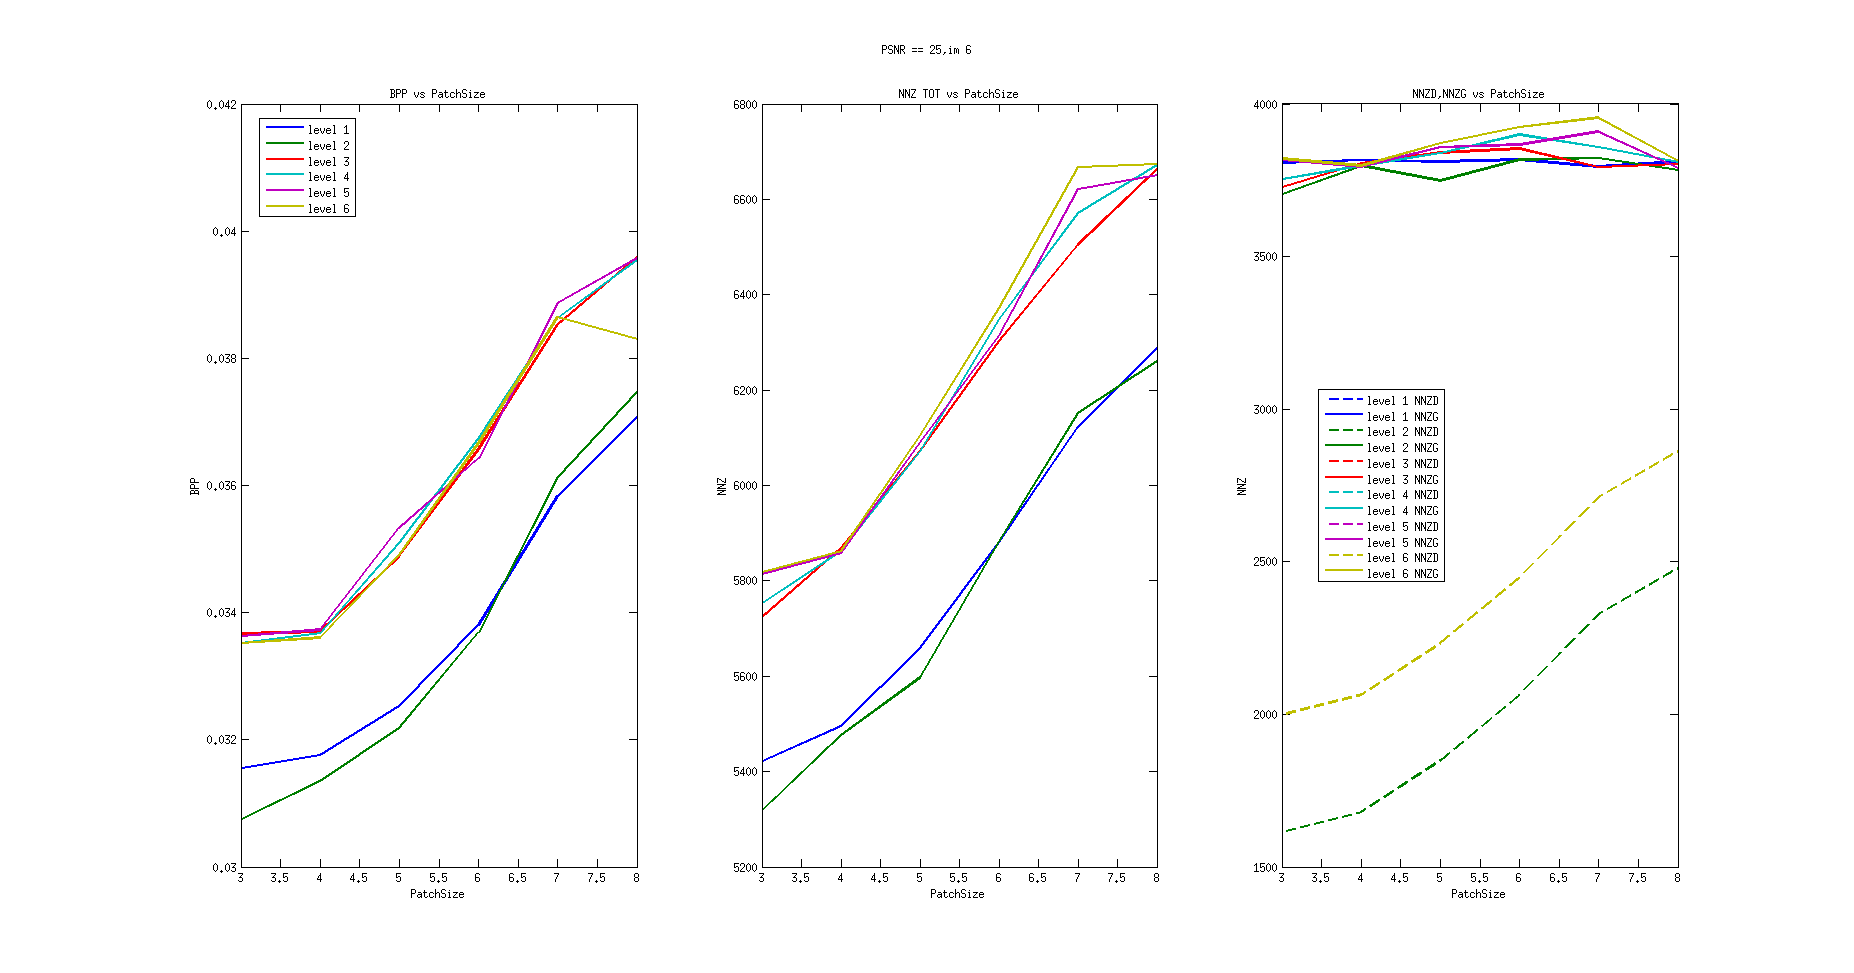
\includegraphics[width=180mm]{fig6L.png}
     
    \end{center}
\end{figure}

\newpage 
\begin{figure}[h]
\centering
    \begin{center}
       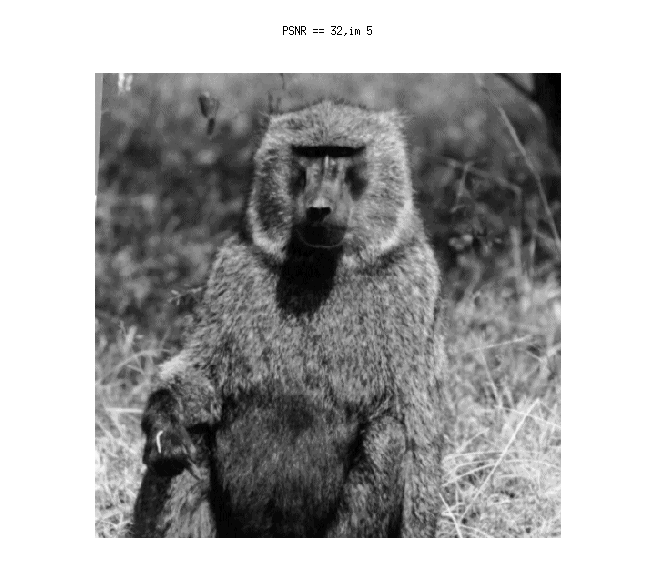
\includegraphics[scale=0.3]{5.png}
    \end{center}
    \noindent
\end{figure}
\begin{figure}[h]
\centering
  
    \begin{center}
       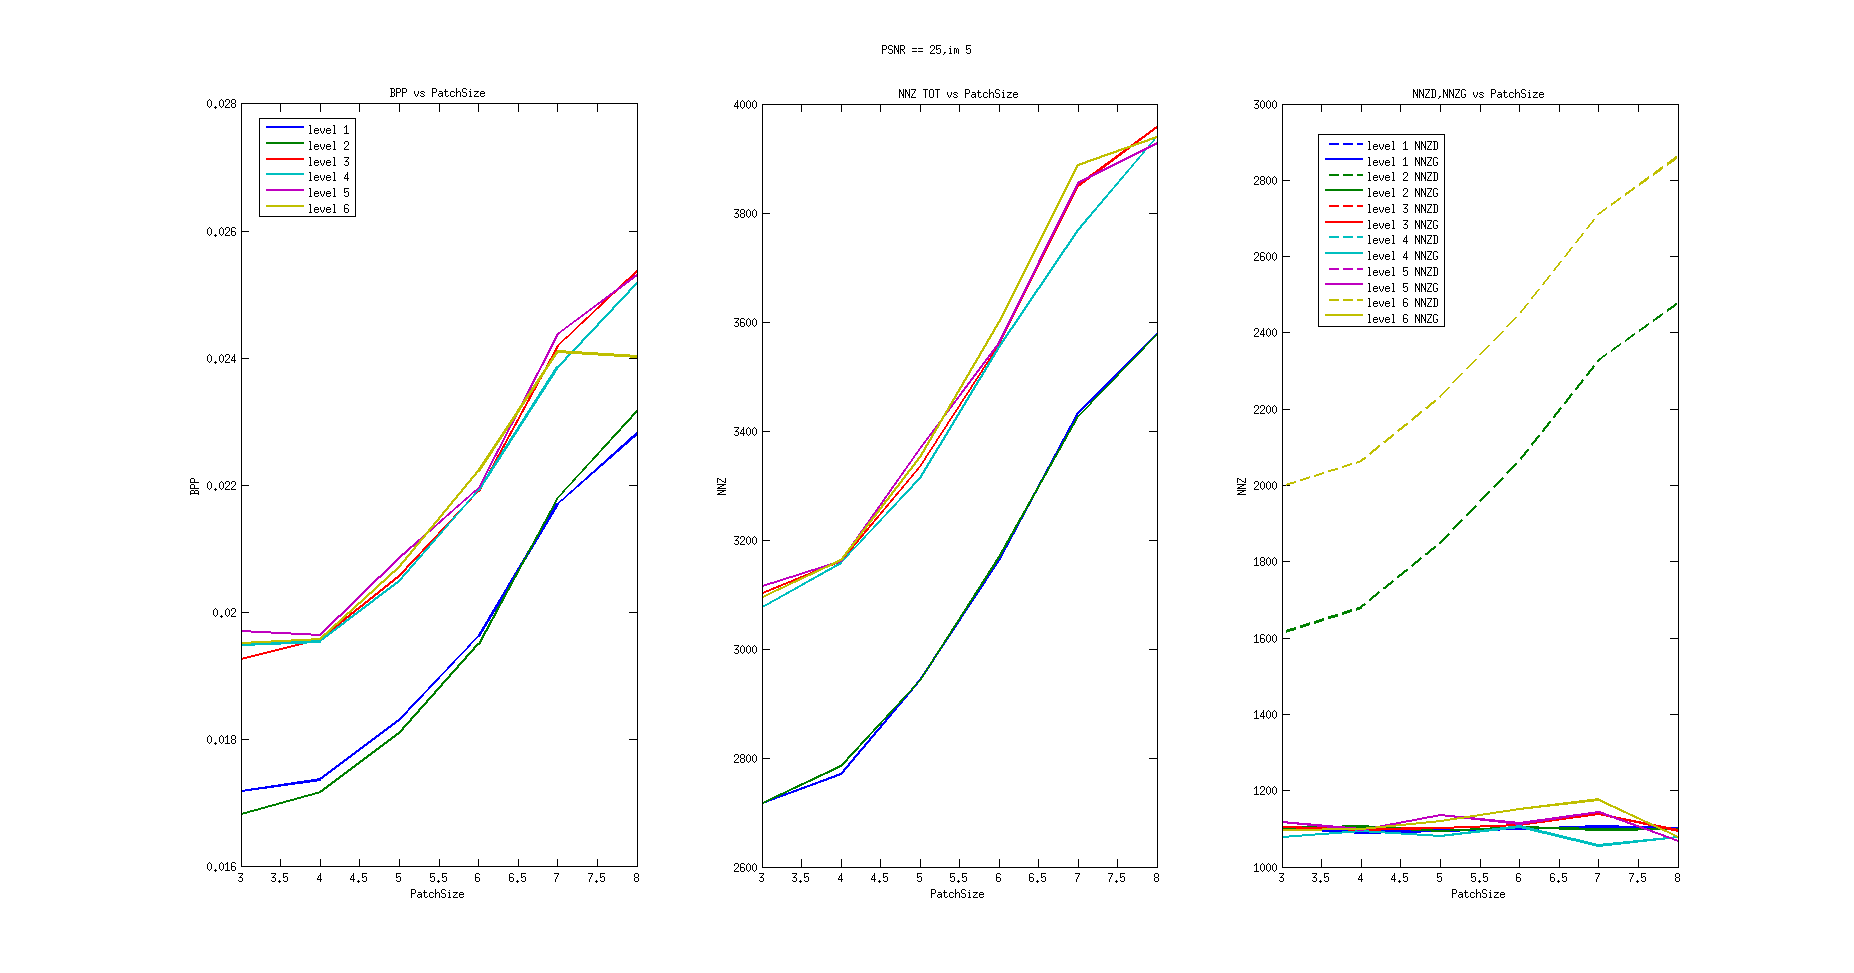
\includegraphics[width=180mm]{fig5L.png}
     
    \end{center}
\end{figure}
Sometimes dictionaries take more space than GAMMAS, as we can see here  big parts of the image has the same characteristics.

\newpage 
\section{PSNR=32 results}
\begin{figure}[h]
\centering
    \begin{center}
       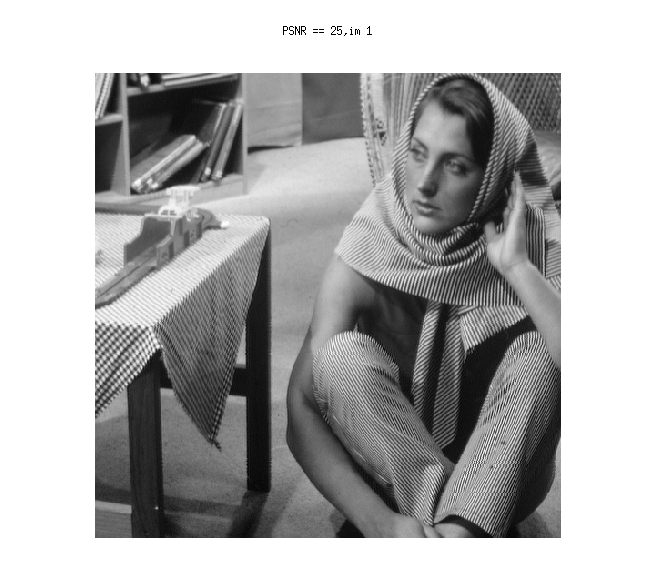
\includegraphics[scale=0.3]{1.png}
    \end{center}
    \noindent
\end{figure}
\begin{figure}[h]
\centering
  
    \begin{center}
       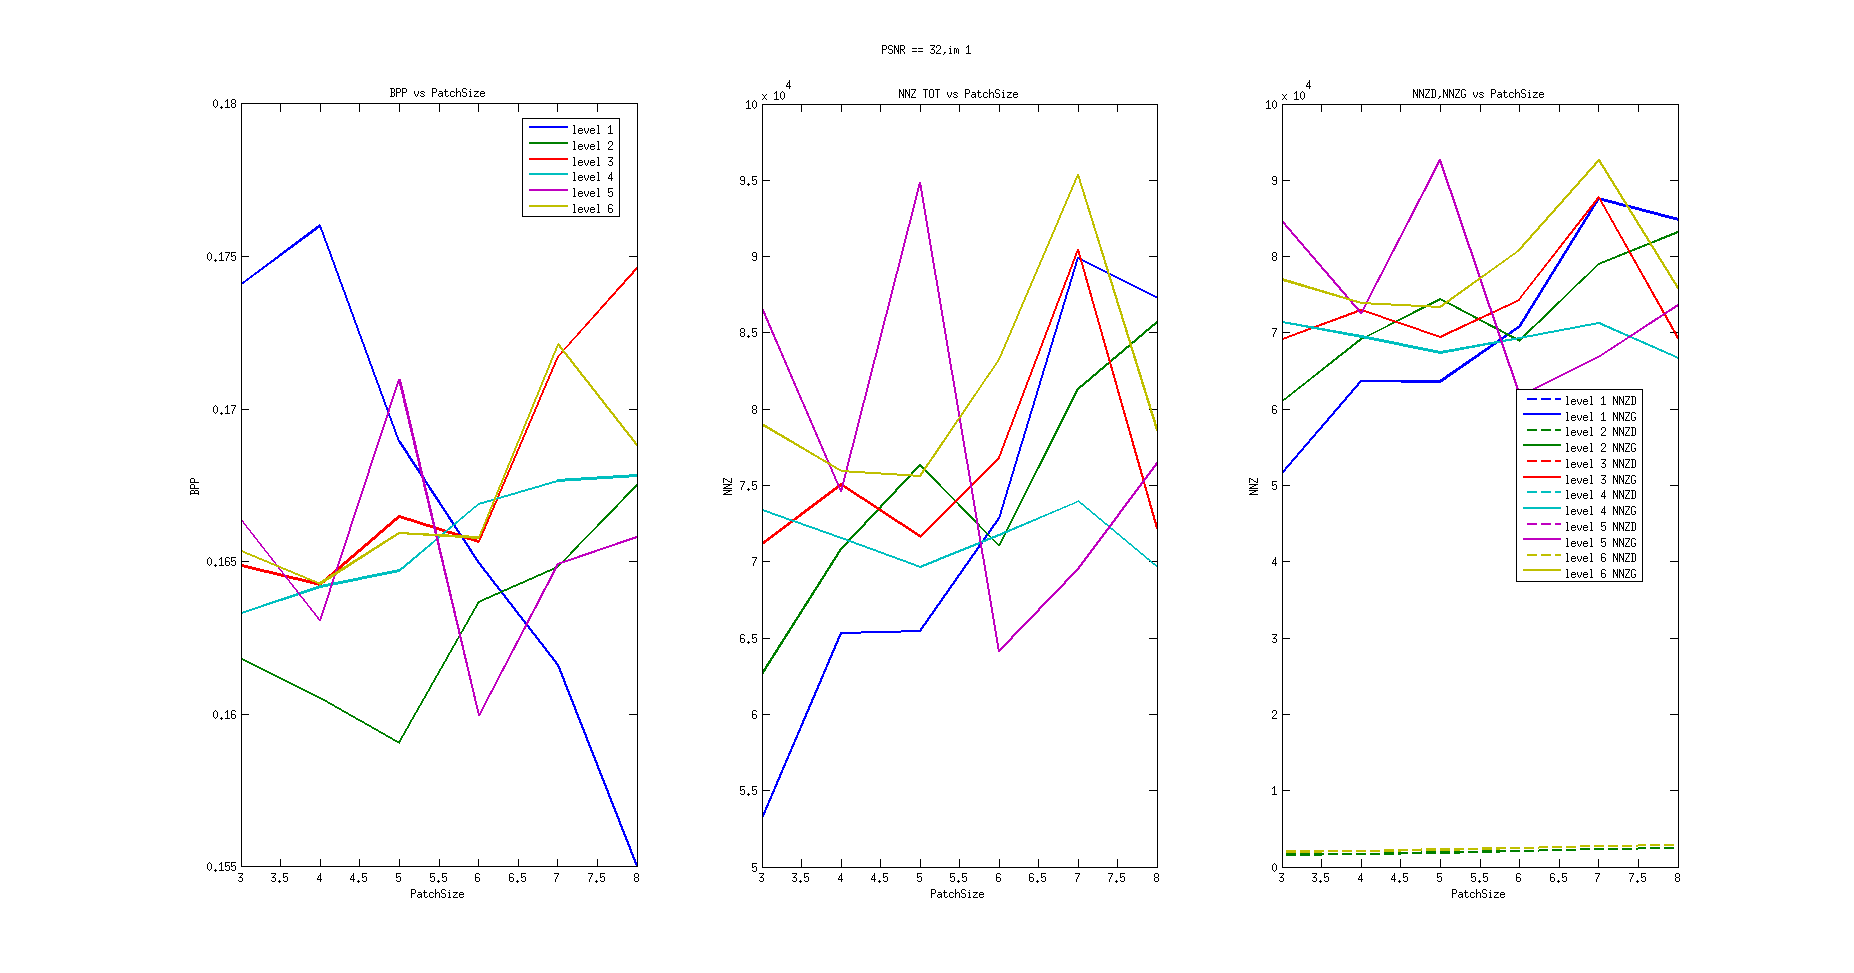
\includegraphics[width=180mm]{fig1H.png}
     
    \end{center}
\end{figure}
here the results is a bit tricky to look at, but generally speaking it seems like lower patch size here tends to be better to, there is a factor that might be seen here, when taking patches ,especially in patch size of an odd number ,there is overhead of zeros padding.

\newpage 
\begin{figure}[h]
\centering
    \begin{center}
       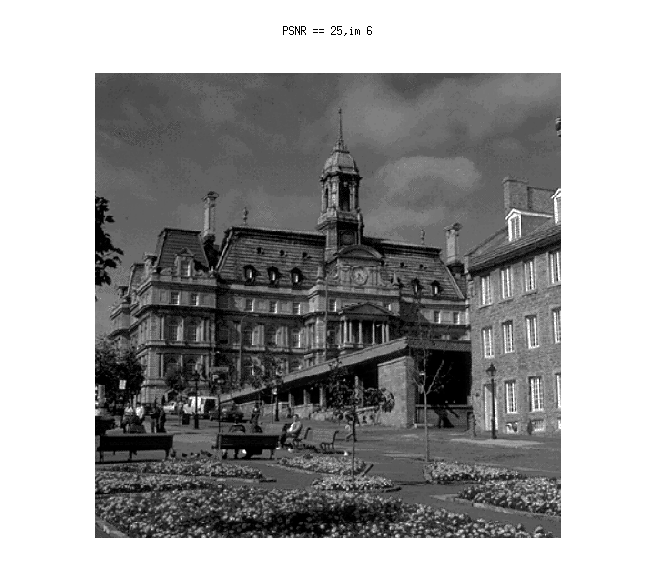
\includegraphics[scale=0.3]{6.png}
    \end{center}
    \noindent
\end{figure}
\begin{figure}[h]
\centering
  
    \begin{center}
       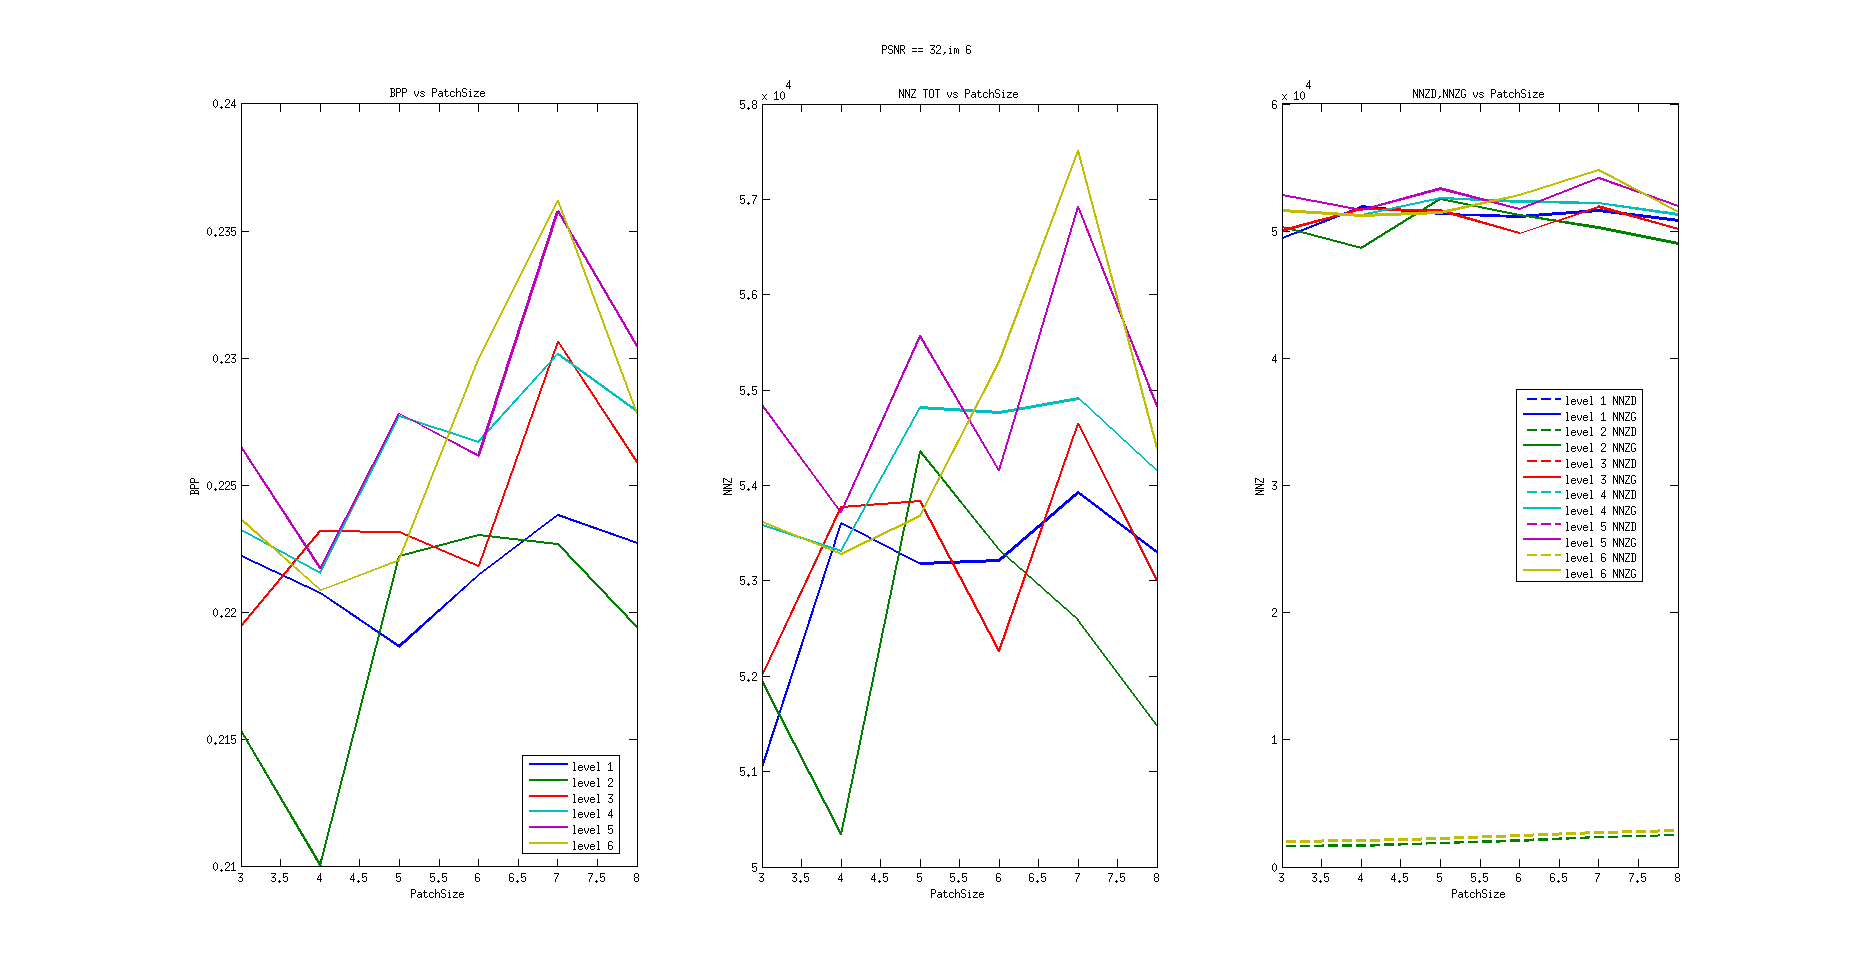
\includegraphics[width=180mm]{fig6H.png}
     
    \end{center}
\end{figure}

\newpage 
\begin{figure}[h]
\centering
    \begin{center}
       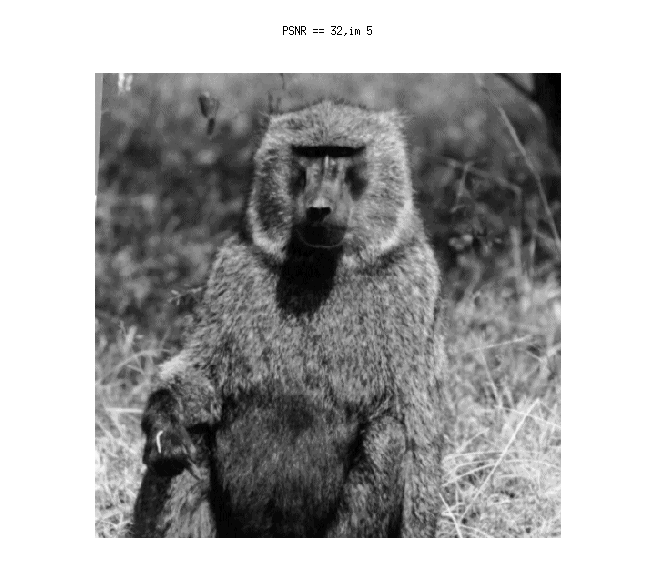
\includegraphics[scale=0.3]{5.png}
    \end{center}
    \noindent
\end{figure}
\begin{figure}[h]
\centering
  
    \begin{center}
       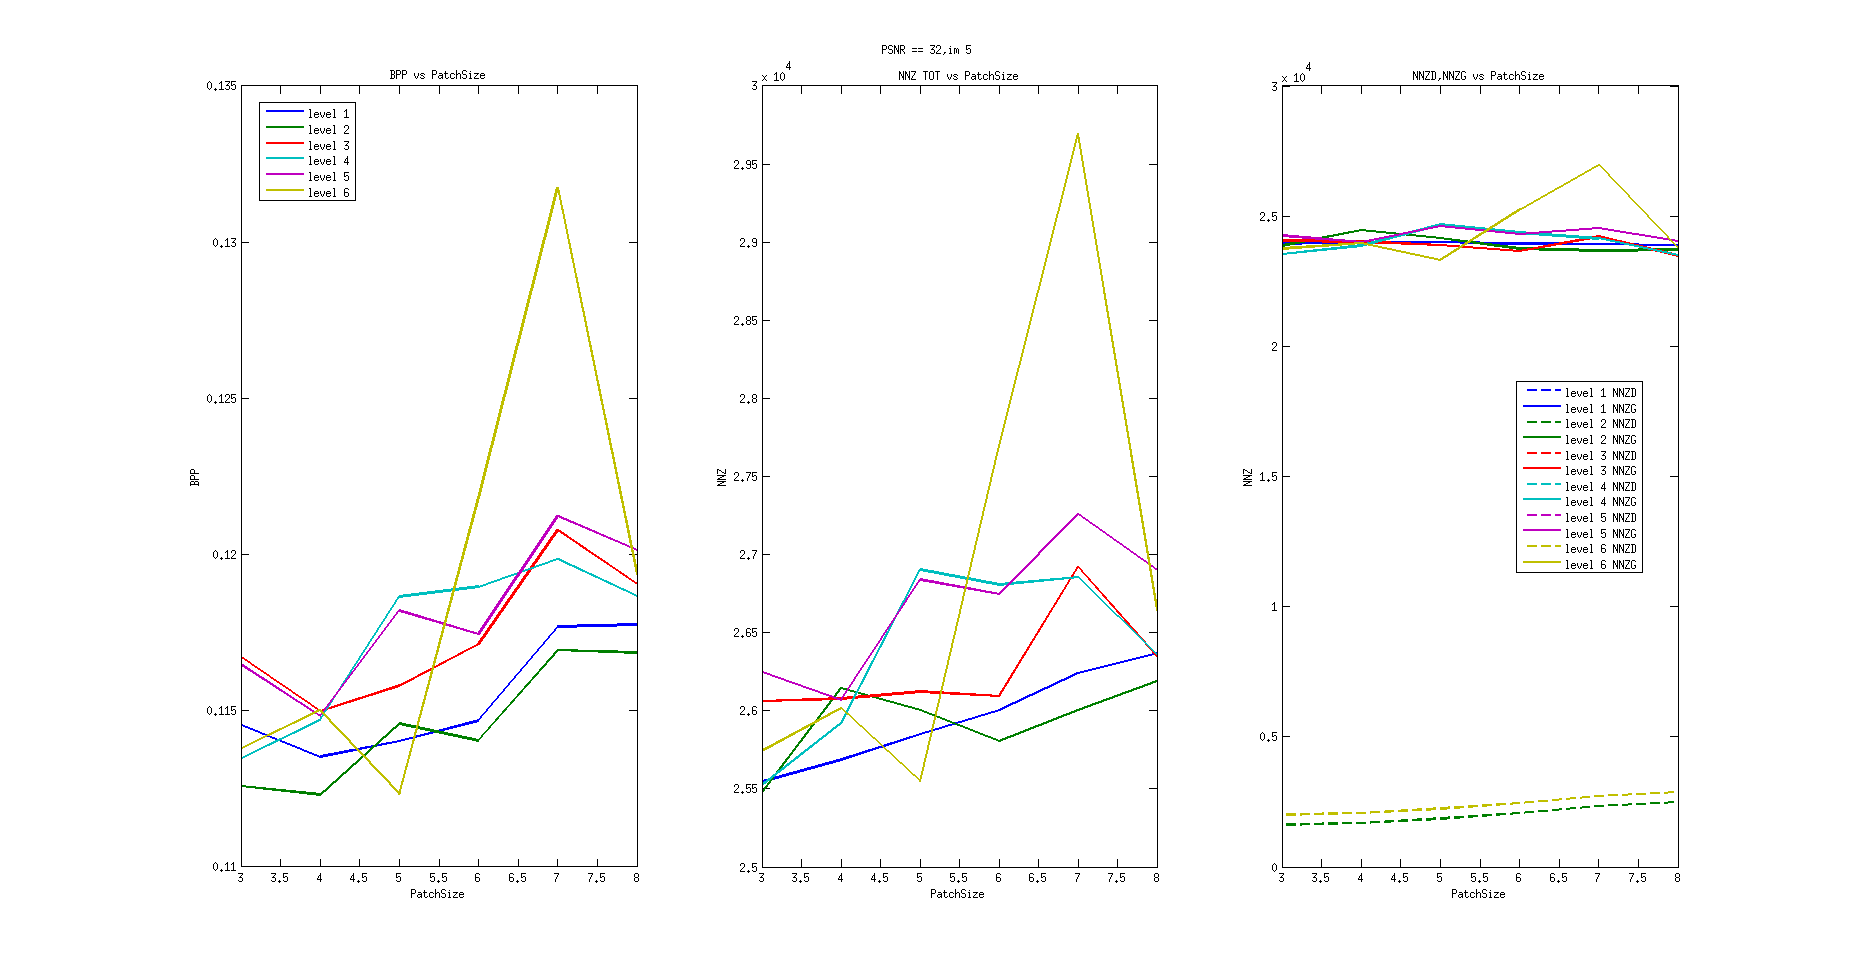
\includegraphics[width=180mm]{fig5H.png}
     
    \end{center}
\end{figure}



\end{document}

